\documentclass[a4paper,english,12pt,bibliography=totoc]{scrreprt}

\usepackage[T1]{fontenc} %immer
\usepackage[utf8]{inputenc} %am
\usepackage{babel} %Anfang

\usepackage{enumitem} %Aufzählungen verändern

%Gleichungen verwenden
\usepackage{newtxtext}
\usepackage{amsmath}
\usepackage{amssymb}
\usepackage{mathptmx}
%\usepackage{txfonts}

\usepackage{listings}% code blocks
\usepackage[most]{tcolorbox}

%Querverweise
\usepackage{varioref} %immer
\usepackage{hyperref} %in dieser
\usepackage{cleveref} %Reihenfolge

\usepackage{booktabs} %schönere Tabellen
\usepackage{siunitx} %SI-Einheiten
\usepackage{tabularx} %Tabellen mit flexiblen Spalten	

\usepackage{graphicx} %Grafiken verwenden

\usepackage{lipsum} %Blindtext
\usepackage{subcaption}
\usepackage{afterpage}
\usepackage[headsepline]{scrlayer-scrpage} %Paket für Kopfzeilen
\usepackage{afterpage}
\usepackage{float}
\automark[subsection]{section}

\usepackage[backend=biber,style=numeric]{biblatex}
\addbibresource{live_cell_imaging.bib} 

\pagestyle{scrheadings}
\ihead{} % oben links
\chead{\leftmark} % oben Mitte
\ohead{} % oben rechts
\cfoot{\pagemark} % unten Mitte
\automark[section]{section} % Modified line

% Zu volle hboxen korrigieren
\tolerance 1414
\hbadness 1414
\emergencystretch 1.5em
\hfuzz 0.3pt
\widowpenalty=10000
\vfuzz \hfuzz
\raggedbottom

%Informationen über das Dokument
\date{\today}


\begin{document}


\begin{titlepage}
	\centering
	
\includegraphics[width=0.8\textwidth]{logo_uulm_sw}
	
	\vspace{1cm}
	\LARGE Laboratory Module for Master Programs
	\Huge \textbf{Biophysics Lab Course}
	
	\vspace{1cm}
	\Large Experiment:

	\Huge \textbf{Live Cell Imaging}
	
	\vspace{15mm}
	\Large Performed on 22.05.2024
	
	\vspace{5mm}
	\LARGE Group 8
	
	\vspace{1cm}
	\Large
	\begin{tabular}{rcl}
	\textbf{Haiyang Zhang} & and & \textbf{Nicolae Turcan}\\
	\href{mailto:student.1@uni-ulm.de}{haiyang.zhang@uni-ulm.de} & & \href{mailto:student.2@uni-ulm.de}{nicolae.turcan@uni-ulm.de}
	\end{tabular}
	
	\vspace{7mm}
	Supervisor: Duyen Huynh
	
	\vfill
	\begin{tabular}{p{50mm}@{\hspace{5cm}}p{50mm}}
	\hrulefill & \hrulefill \\
	%\centering Haiyang Zhang  & \centering Nicolae Turcan
	\end{tabular}
	
	\vspace{5mm}
	\normalsize \raggedright
	We hereby confirm that we have elaborated the present work independently and have detailed knowledge of the entire contents.
\end{titlepage}



\tableofcontents

\chapter{Introduction}
\label{cha:Introduction}
%in depth description of the instrument, spinning disc confocal setup no longer than 1 page 
The following report contains a series of experiments with the aim of understanding the dynamic biology of live cells.
The technology used is a form of fluorescence microscopy, where fluorescent reporters are used to increase contrast between the phenomenon of interest and the surrounding background. The instrument  that enabled our investigation was the Spinning Disk Confocal Microscope.\\
\newline
The Spinning Disk Confocal Microscope is a type of confocal Microscope, that employs the confocal principle in a novel way, enabling much faster frame rates, which make it ideal for recording at a time scale compatible with biological processes, while still mantaining a resolution that enables meaningful insights on the molecular processes that govern cell dynamics.
\newline
Fluorescence of a marker molecule coupled with the object of interest is the first method used to gain contrast, but it´s still susceptible to out of focus light, this issue is overcame with a confocal set-up.\newline
A confocal set-up consists in the use of a pin-hole aperture ( roughly on the same size of the emission wavelength) to remove the light out of focus \cite{confocal}, the pinhole is positioned at the rear focal plane of the microscope objective, this allows to block any light coming from outside the front focus point of the objective, effectively reducing the volume which produces the image to femtoliters (depending on pinhole diameter and magnification of objective). This effectively increases the resolution of the microscope by decreasing the voxel size to the femtoliter scale,the pinhole lets only intensity information of the image go trough, and no spatial information is preserved if $\lambda$ $\sim$ pinhole 
diameter )  and as expected also increase dramatically the image acquisition time, because to produce an image we need to acquire intensity values over the whole span of XYZ axes with a single point.\newline
To counteract the extremely long acquisition time, an array of pinholes can be used to achieve simultaneous acquisition over multiple points in the XY plane, the pinholes still require to be distant enough from each other to avoid constructive interference in the projected image, but the acquisition speed is increased linearly by the number of pinholes simultanously employed.The pinhole array is arranged on a Nipkow´s disk\cite{Spinning_disk}, that rotates to produce the scanning action, thus the name Spinning Disk Confocal Microscope.\\
\newline
An optical diagram of the set-up is presented in Figure 1.1 to visually support the introduction on the instrument.

\begin{figure}[H]
    \centering
    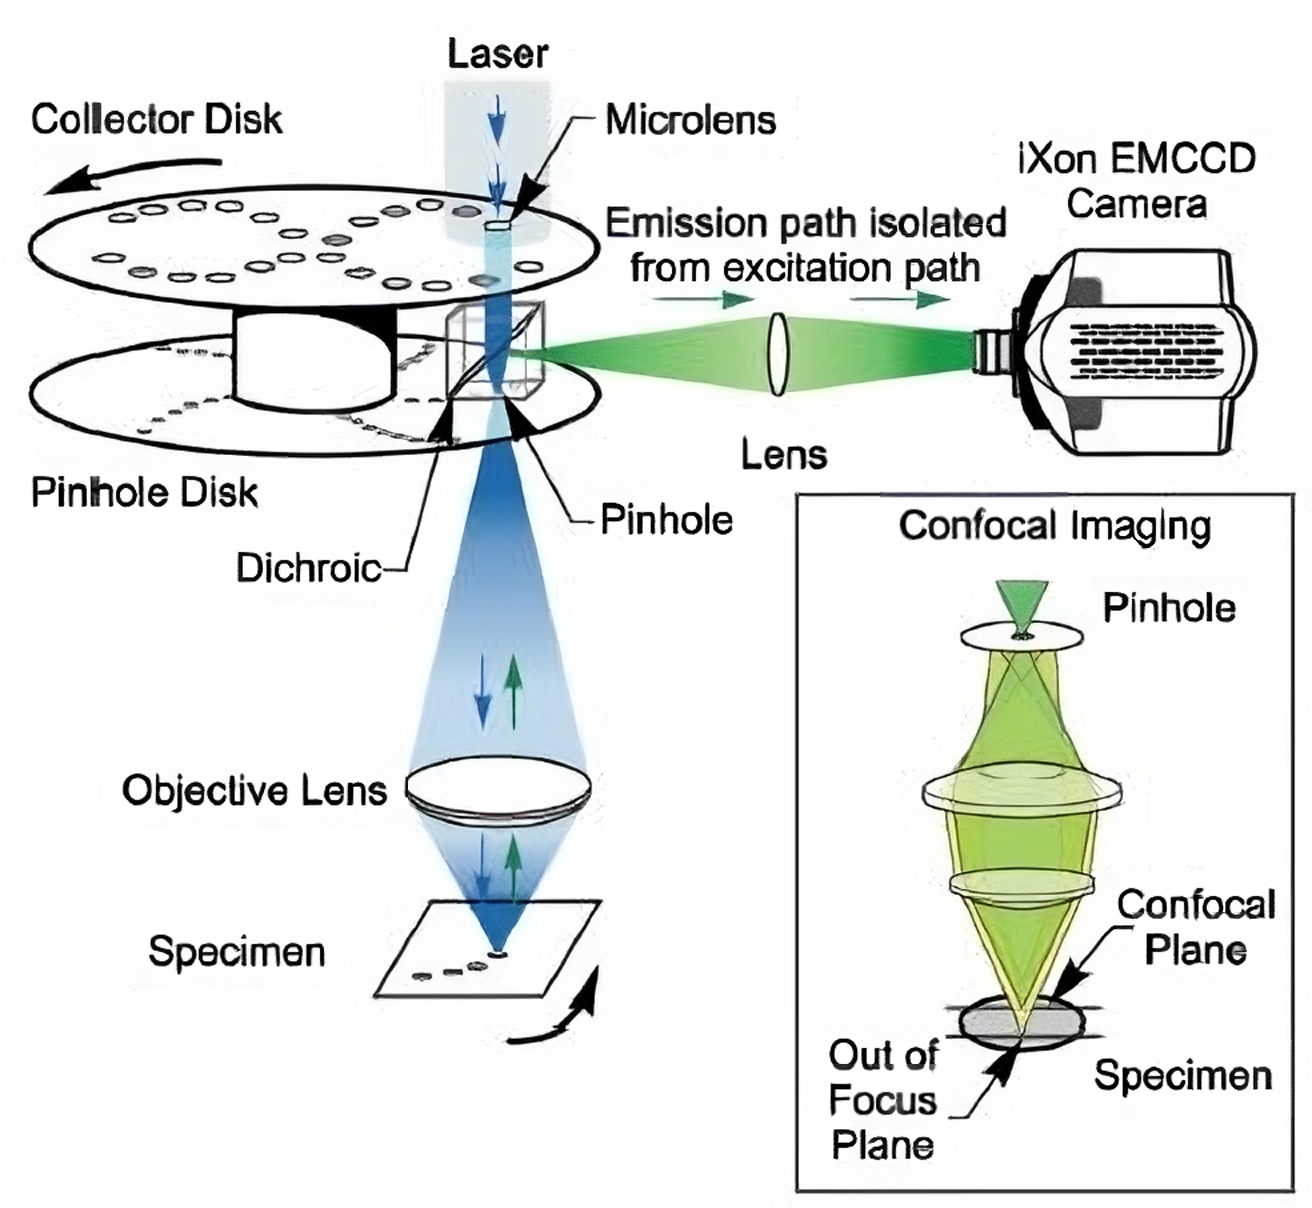
\includegraphics[width=0.99\textwidth]{Images/Spinning Disk Confocal Setup.jpeg}
    \caption{The Spinning Disk Confocal Microscope with detail of Confocal principle\cite{Spinning_disk}}
    \label{fig:enter-label}
\end{figure}





\chapter{Rhodamine-Phalloidin Staining of HeLa Cells}
\label{cha:Experiment1}
\section{Experiment}
%short description of experiment, a few phrases
This experiment is aimed to label the actin filaments of HeLa cells using the rhodamine-phalloidin staining. Phalloidin can effectively bind to F-actin, which is the subunit of the actin filament and can be coupled to different fluorescent dyes like rhodamine. In this experiment, the cells(HeLa) were fixed and permeabilized first, then we applied rhodamine-phalloidin to label the actin filaments. After that, the sample was observed under a confocal fluorescence microscope with a 532nm laser. A z-stacks movie(steplength = 500nm, 61 frames in total) was captured from out of focus$\xrightarrow{}$ in focus$\xrightarrow{}$out of focus. Then the z-stacks movie was used to make the 3D view of the cells enabling us to observe the actin distribution from the images.
\section{Results}
%show Z stack of cell
%light is renormalized and doesn't show the real intensity.
%why we still see out of focus light
The captured figures are shown below(from Figure 2.1 to Figure 2.6). The fluorescence signals were shown in red, and in this experiment they showed the positions of the actin filaments.\\
\begin{figure}[htbp]
    \begin{minipage}[t]{0.5\linewidth}
        \centering
        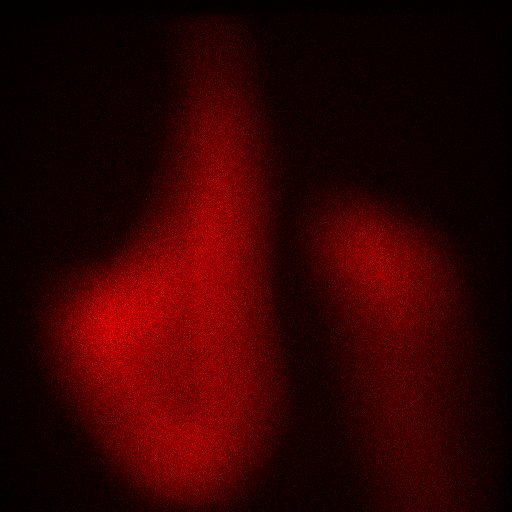
\includegraphics[width=0.9\textwidth]{Images/Actins/Actin_zscan_500nm_10.jpg}
        \caption{The 10th frame of the\\ z-stacks movie}
    \end{minipage}%
    \begin{minipage}[t]{0.5\linewidth}
        \centering
        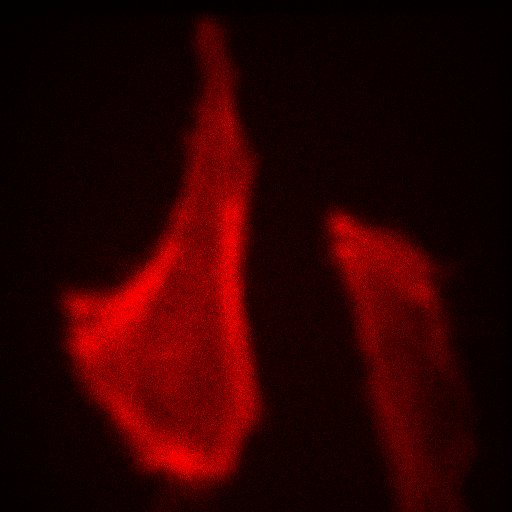
\includegraphics[width=0.9\textwidth]{Images/Actins/Actin_zscan_500nm_20.jpg}
        \caption{The 20th frame of the\\ z-stacks movie}
    \end{minipage}
\end{figure}

\begin{figure}[htbp]
    \begin{minipage}[t]{0.5\linewidth}
        \centering
        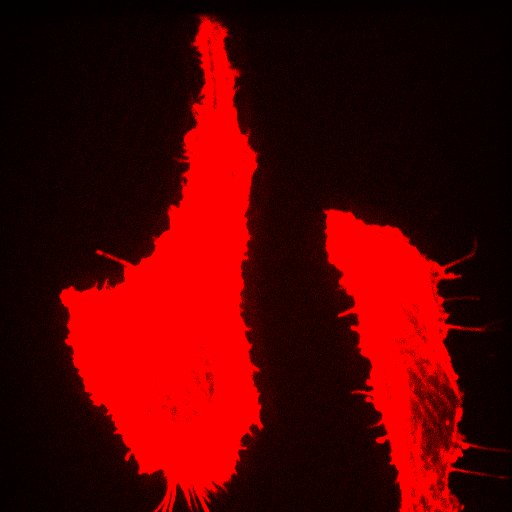
\includegraphics[width=0.9\textwidth]{Images/Actins/Actin_zscan_500nm_30.jpg}
        \caption{The 30th frame of the\\ z-stacks movie}
    \end{minipage}%
    \begin{minipage}[t]{0.5\linewidth}
        \centering
        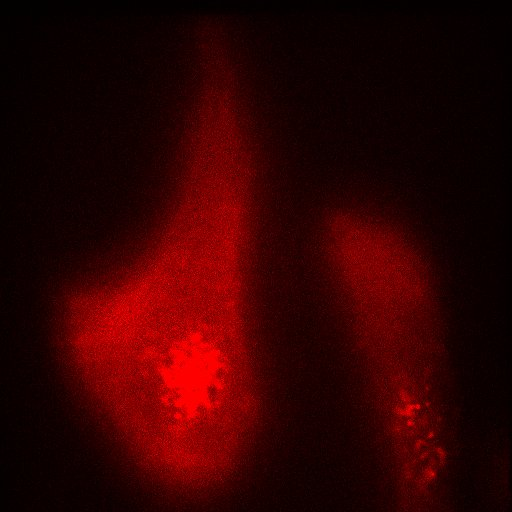
\includegraphics[width=0.9\textwidth]{Images/Actins/Actin_zscan_500nm_40.jpg}
        \caption{The 40th frame of the\\ z-stacks movie}
    \end{minipage}
\end{figure}

\begin{figure}[htbp]
    \begin{minipage}[t]{0.5\linewidth}
        \centering
        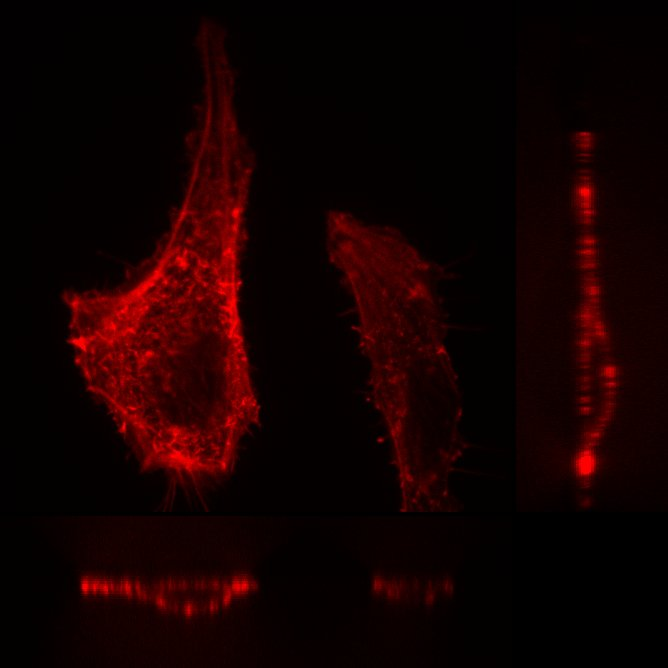
\includegraphics[width=0.9\textwidth]{Images/Actins/Orthogonal_slice_view.jpg}
        \caption{The orthogonal slice of the\\ HeLa cell and the actin \\cytoskeleton}
    \end{minipage}%
    \begin{minipage}[t]{0.5\linewidth}
        \centering
        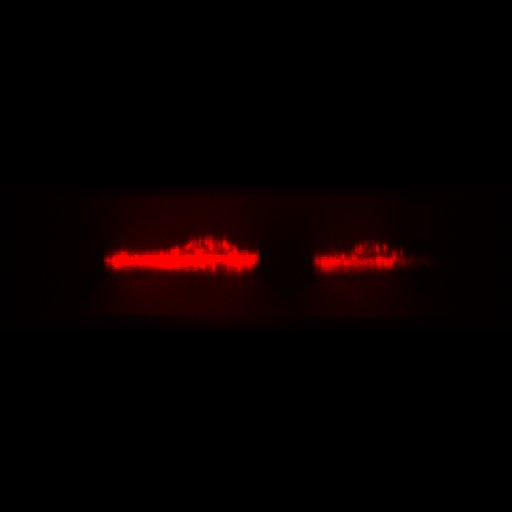
\includegraphics[width=0.9\textwidth]{Images/Actins/zscan 3D View.jpg}
        \caption{The 3D view of the HeLa cell \\and the actin cytoskeleton}
    \end{minipage}
\end{figure}

Figures 2.1 to 2.4 show four frames of the Z-stacks movie. The hazy images were captured from out-of-focus planes, while the bright images were captured from focused planes.\\


Figure 2.6 is the 3D reconstruction of the cell, while Figure 2.5 is the orthogonal slice of the HeLa cell. In Figures 2.5 and 2.6, we proceed with an intensity normalization that allowed us to observe the distribution of the actin filaments in the cell much more clearly. 


\section{Discussion}
%discuss by Nyquist Sampling Rate, morphology of the actin filaments(cell), filopodia


\begin{figure}[H]
    \centering
    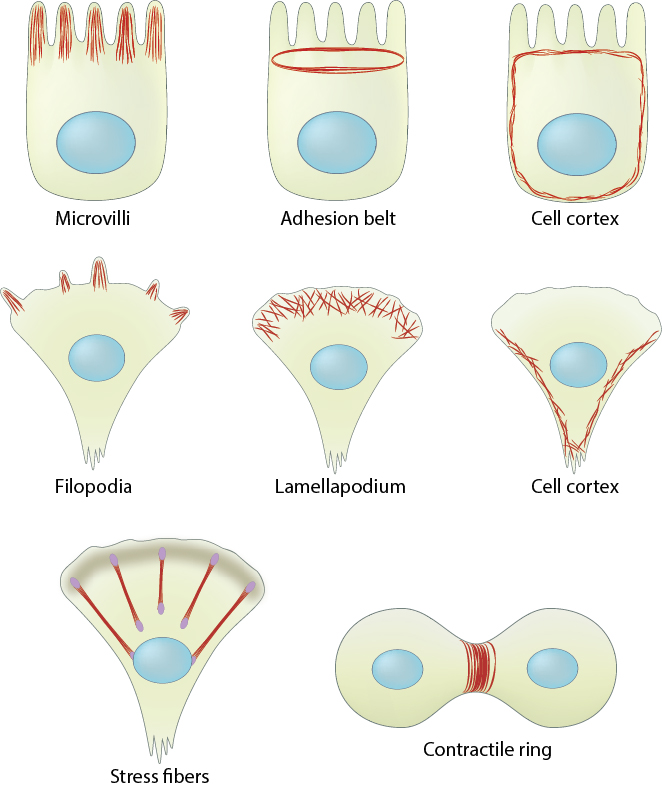
\includegraphics[width = 0.8\textwidth]{Images/Actins/actin-filament-distribution.jpg}
    \caption{Reference Image for Actin quaternary structures\cite{Actin_quanternary_structures}}
    \label{fig:enter-label}
\end{figure}

Several types of actin quaternary structures could be noticed from the fluorescence images of the cell. In Figure 2.5, we can observe Lamellapodium(the broad and sheet-like distribution of the short actin filaments near the membrane), cell cortex(the thin actin filament wrapped around the cell), and filopodia(the finger-like protrusions extending from the cell surface). The dark part in the middle of the cell images could be the nucleus since there are no actin filaments inside the nucleus. A reference image that helped us recognize the various structures is provided in Figure 2.7\\

In this experiment, the image intensity in the red channel does not equal to the real intensity of the fluorescence. Instead, it is a normalized intensity to help us find the focal plane of the objective. And the hazy images of the z-stacks movie are from the out-of-focus light from the fluorescence. The shift on the x and y-axis of the fluorescence will be blocked out by the pinhole, while the shift on the z-axis still allows some of the light to go through the pinhole, as suggested in the cases of a and b in Figure 2.8, however still with a much lower intensity, the decrease in light intensity can also be sensed from the grainier nature of the images, which is a direct result of the a smaller intensity range or higher sensor gain.

\begin{figure}[H]
    \centering
    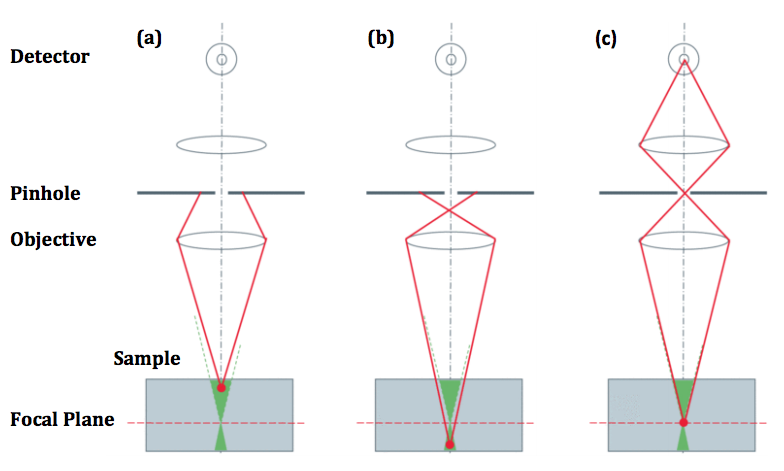
\includegraphics[width = 0.8\textwidth]{Images/confocal microscopy.png}
    \caption{Confocal microscopy with out-of-focus light coming for axial light of z-axis \cite{confocal}}
    \label{fig:enter-label}
\end{figure}

\chapter{Detection of $\mathbf{ca^{2+}}$ Oscillations in HeLa Cells in Response to Various Stimuli}
\label{cha:experiment2}

\section{Experiment}
%histamine and then ionomycin
This experiment is aimed to investigate $\mathrm{ca^{2+}}$ oscillations in HeLa cells in response to histamine and ionomycin using the calcium-sensitive fluorescent dye Fluo-4.\newline
We incubated the cells with Fluo-4 modified with acetoxymethyl to enable it to cross the plasma membrane, it becomes fluorescent upon binding $\mathrm{ca^{2+}}$, allowing visualization of intracellular $\mathrm{ca^{2+}}$ dynamics. After some washing steps we proceded by focusing on some healthy cells and then providing histamine at a known concentration in the extracellular solution ,we repeated this step with concentrations of 2µM, 10µM and 50µM Histamine.\newline
Histamine is a signaling molecule that activates transmembrane G-Protein Coupled Receptors, which in turn causes a release of $\mathrm{ca^{2+}}$ from the Endoplasmic Reticulum into the cytoplasm ( see Figure 3.2 ) . In the meanwhile Sarcoplasmic ATPases constantly re-sequester $\mathrm{ca^{2+}}$ back into the ER, and when the Histamine Signal is successfully transduced again, it causes again another rapid release of Ions as described above.\cite{lee_mechanisms_2001}\newline
Subsequently, we treated all cells with a solution of Ionomycin ( see Figure 3.1  for evident anphipatic nature of molecule) and 4µM $\mathrm{ca^{2+}}$, which acts as Ionophore capable of moving across all membranes, this induces rapid $\mathrm{ca^{2+}}$ release from intracellular stores at speeds compatible with simple diffusion and where no cellular signal transduction is required, providing a maximal fluorescence signal for normalization.
\begin{figure}[H]
    \centering
    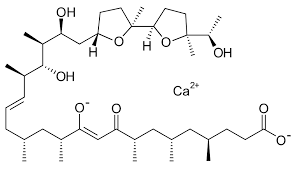
\includegraphics[width=0.25\linewidth]{Images/Ionomycin.png}
    \caption{Ionomycin molecule with bound Ion}
    \label{fig:enter-label}
\end{figure}


\section{Results}
The Following Figures display Fluorescence Intensity over Time ( expressed as Mean Value over Frame ) for some selected ROIs, corresponding to background and the cells in frame.

\begin{figure}[H]
    \centering
    \includegraphics[width=0.8\linewidth]{Images/Calcium/Intensity_Plot_Ca_His_2µM_data_BG_6Cells.png}
    \caption{Intensity Plot at 2µM Histamine Background + 6Cells and Ionomycin}
    \label{fig:enter-label}
\end{figure}    

    \begin{figure}[H]
    \centering
    \includegraphics[width=0.8\linewidth]{Images/Calcium/Intensity_Plot_Ca-His_10µM_data_BG+4Cells.png}
    \caption{Intensity Plot at 10µM Histamine Background + 4Cells and Ionomycin}
    \label{fig:enter-label}
\end{figure}

    \begin{figure}[H]
    \centering
    \includegraphics[width=0.8\linewidth]{Images/Calcium/Intensity_Plot_Ca-His_50µMdata_3Cell_BG_SUBSTACK.png}
    \caption{Intensity Plot at 50µM Histamine 3 Cells + Background}
    \label{fig:enter-label}
\end{figure}
    
%The intensity-time curve to show the oscillation(and some dark and light images).  

Figure 3.5 evidences the importance of time-resolution enabled by the spinning disk set-up, since otherwise this process couldn´t be imaged, It represents intensity over time for concentric ROIs around the putative position of the ER in the cell, where the Ions are released from.

    \begin{figure}[H]
    \centering
    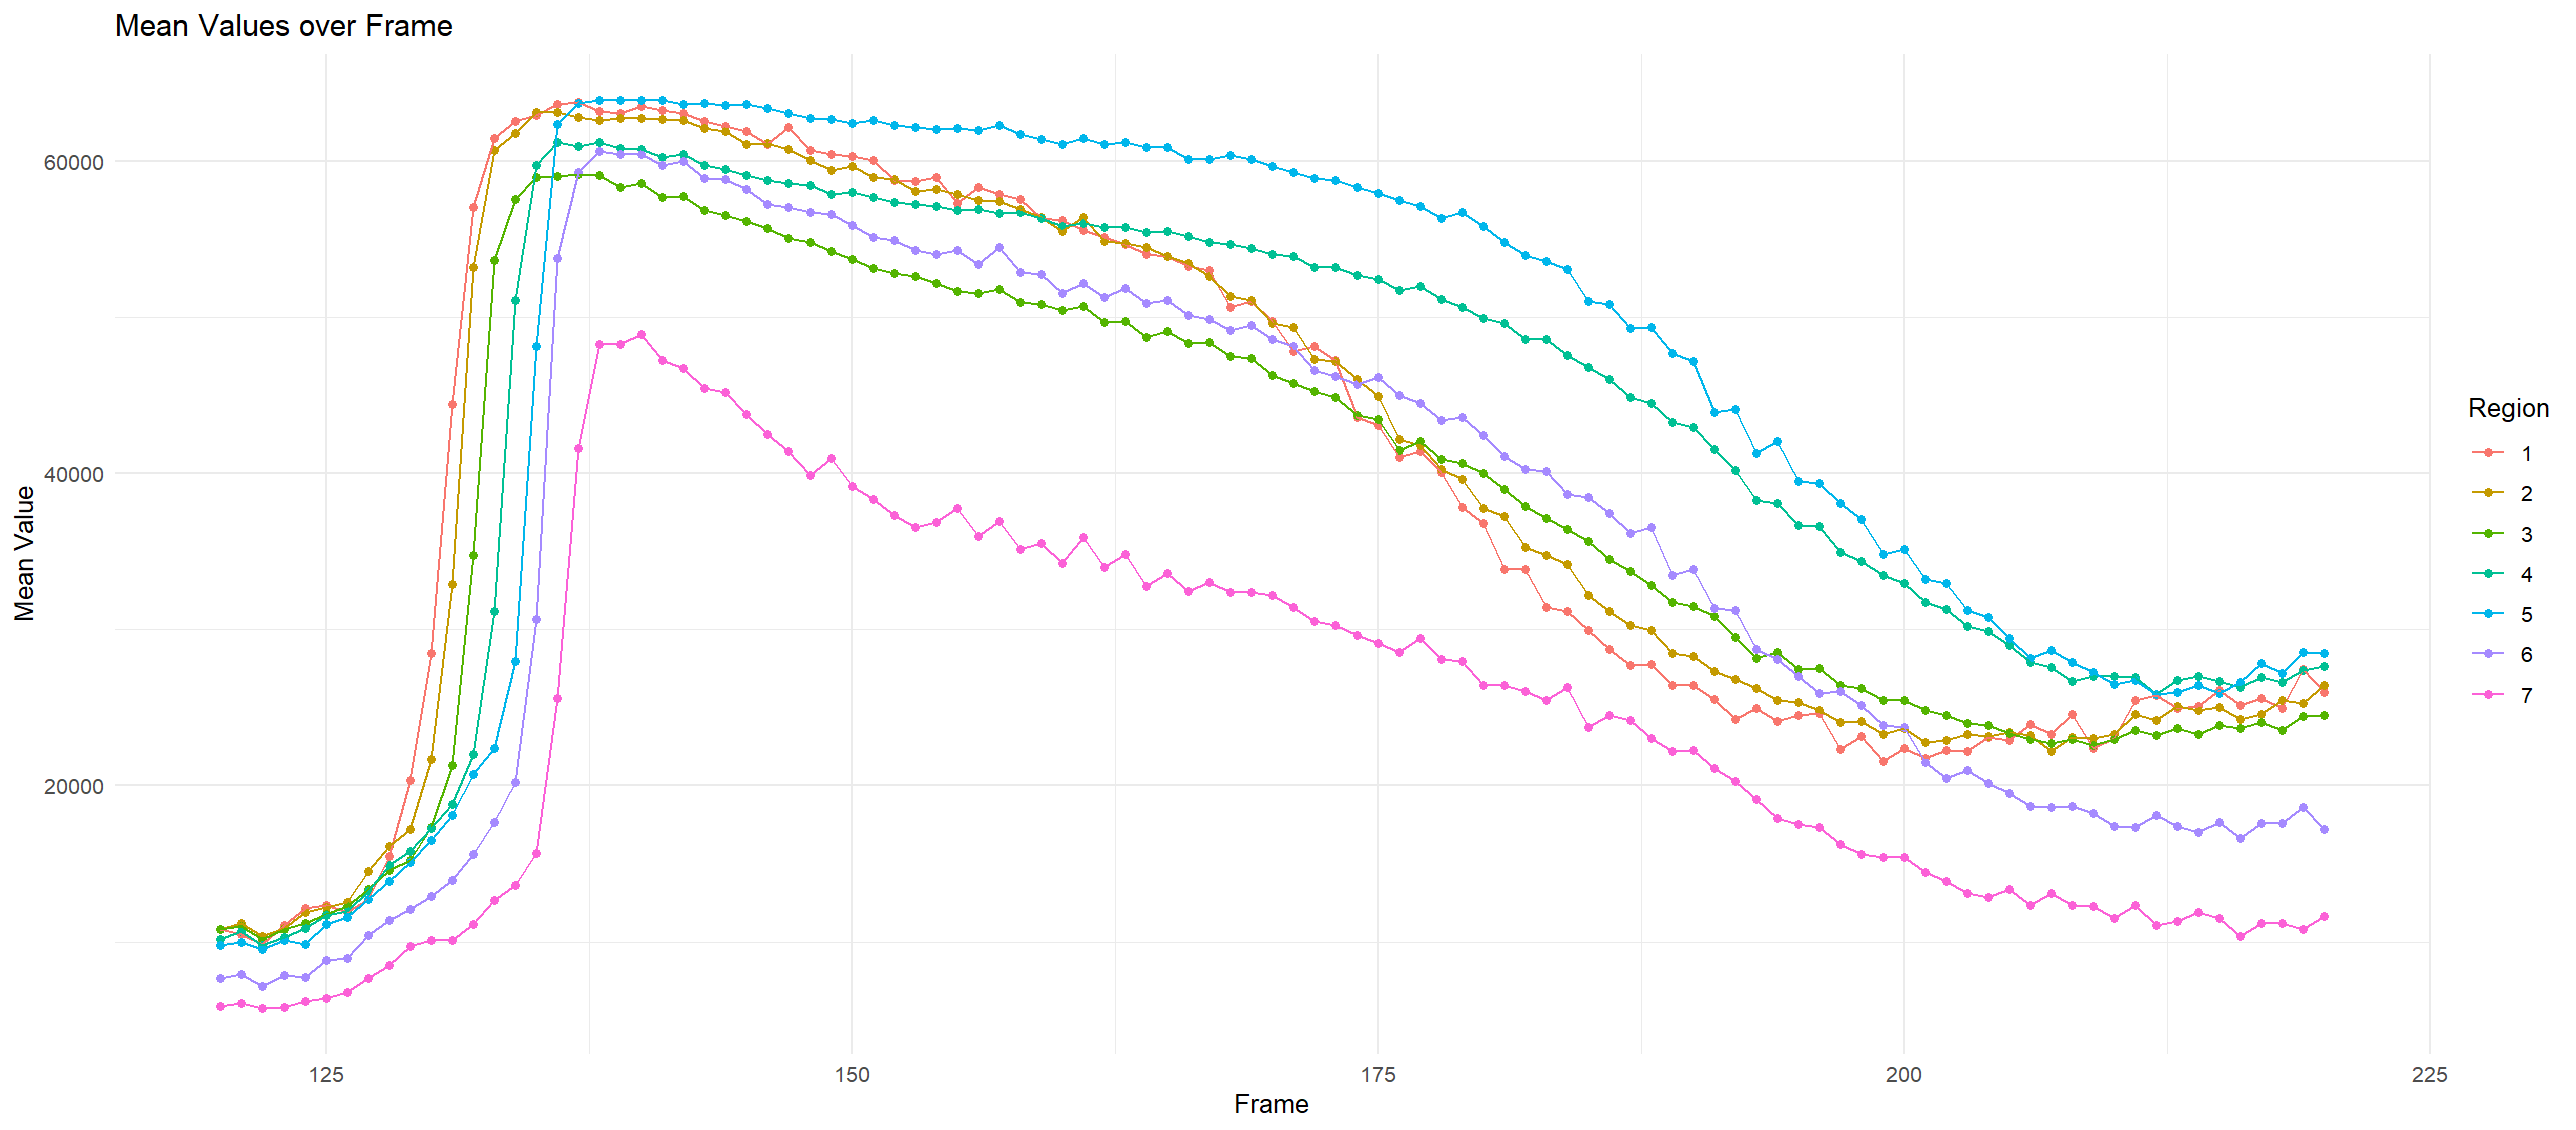
\includegraphics[width=0.9\linewidth]{Images/Calcium/Time Delay Because of Diffusion.png}
    \caption{Time delay in Intensity Increase based on distance from ER }
    \label{fig:enter-label}
\end{figure}

Figure 3.6 displays 8 Frames ( 130- 137 ) that clearly show the diffusion of $\mathrm{ca^{2+}}$ and underline the speed of biological processes and the importance of a high frame-rate setup capable of recording such processes. The cell on the bottom right display especially well the region from where the Intensity increases first, enabling us to putatively recognize that region as the position of the ER in the Cell without directly staining for it.

    \begin{figure}[H]
    \centering
    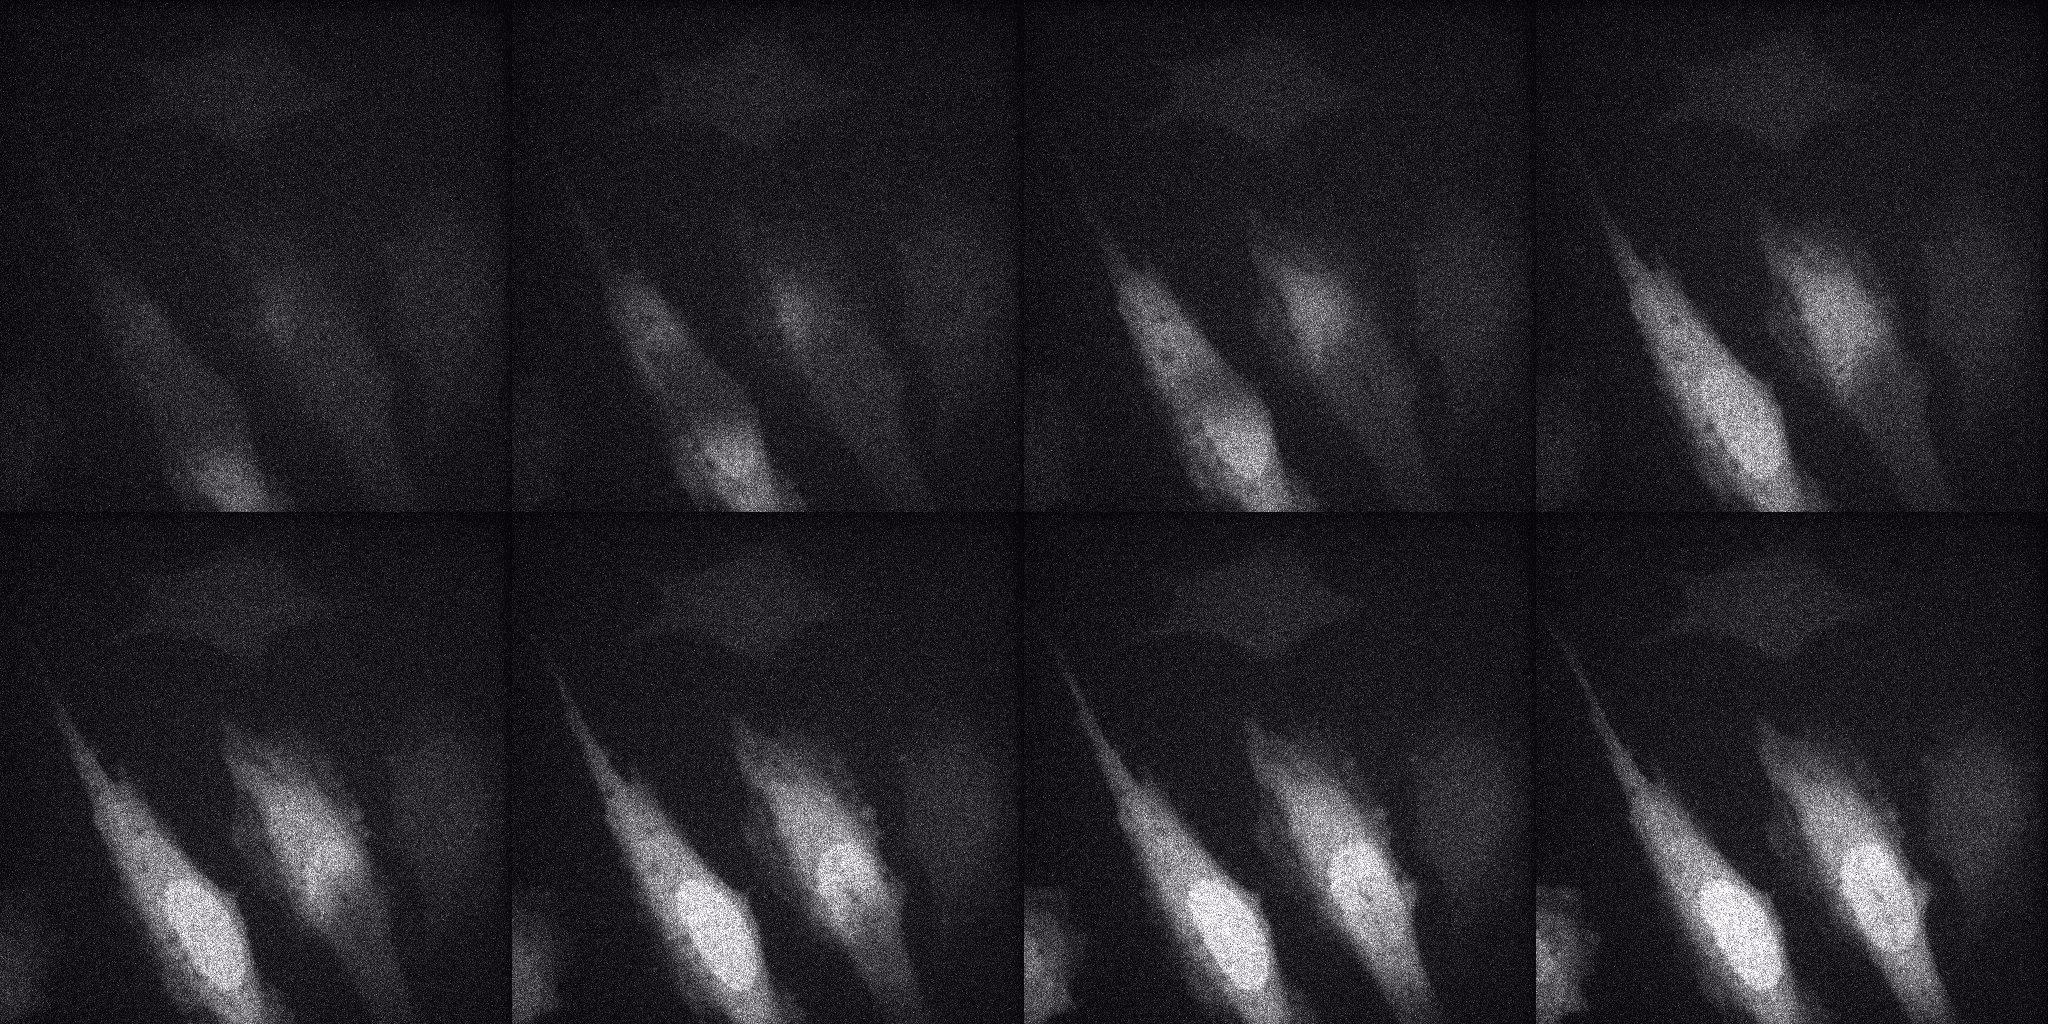
\includegraphics[width=0.9\linewidth]{Images/Calcium/Diffusion Frames.jpg}
    \caption{Frames 130 to 137 }
    \label{fig:enter-label}
\end{figure}

\section{Discussion}

Figure 3.2 clearly shows that the first increase in intensity is almost simultaneous for all imaged cells. This can be interpreted as the fact that after the addition of the 2µM Histamine Solution, it quickly diffused everywhere in the medium and that the 
first peak corresponds to a signal transduction cascade highly conserved through all the cells imaged. This results in all the cells being initially in phase
and subsequently moving out of phase with each other ( as clearly displayed by the traces of the Cells 4 and 5 ).\newline
We argue that the reason why the oscillations after the first one are out of phase is that restoring the "ready-state" of the signal transduction pathway is much more susceptible to stochastic fluctuations, this could be because the number of proteins required to collaborate to restore the state is much larger, and the specific amounts of proteins that make up this system vary greatly between single cells, therefore reaction rates and time have a much greater weight in influencing subsequent peaks.\newline
\\
The Cells displayed in Figure 3.2 were treated with Ionomycin and a 2µM $\mathrm{ca^{2+}}$ but it didn´t provide a sufficient signal for normalization. 
%fluorescence of Ionomycin in example 1 didn´t make sense because the concentrations between cytosol Ca2+ and ER were very different, why should an increase in ca2 solution of Ionomycin make such a big difference?? 
Figure 3.3 displays the clearest results of the data we acquired. The first intensity peaks are contemporary except for a shifted one, which was the result of the 4the cell being further downstream the well channel and a delay equal to the time necessary for simple diffusion to reach it, Figure 3.6 displays the reason for this delay very clearly.\newline
The other peaks display the out-of-phase oscillations discussed above even with more clarity and finally, the last increase in intensity  and subsequent plateau is the result of the Ionomycin treatment.
The  Ionomycin treatment was 5µM with an additional 4µM $\mathrm{ca^{2+}}$ to compensate for the previous failure in achieving a clear Ionomycin increase in intensity.\\

The reason why the Calcium Ion concentration in the Ionomycin treatments of Figure 3.2 and Figure 3.3 resulted in such a different response in fluorescence intensity still escapes our current comprehension of the ionophore activity.\\

%3rd sample was moved( by nicolai by mistake) 2nd sample was the best one
We would like to note that Figure 3.4 doesn´t show the Ionomycin treatment because the recorded field of view was mistakenly moved during the application of the solution, thus there is no plateau of Intensity for normalization purposes such as in Figure 3.3\\
% the time between cycles after histamine varies for each cell, because it depends on the internal signal transduction pathways of each cell, where as for Ionomycin, all cells act simultaneously because the ionophore just makes it into passive diffusion, not controlled by the cell anymore.

% why is Calcium brighter in Nucleus?
It is clear from the figures presented that nuclear Fluo4 fluorescence was consistently higher than cytosolic fluorescence, even after both signals had recovered. This difference is due to the inherent brightness of fluo4 in the nucleus compared to the cytosol, rather than a sustained $\mathrm{ca^{2+}}$ gradient between the cytosol and nucleus\cite{bootman_update_2009}. This could be the result of a more acidic environment in the nucleus acting on Fluo4 fluorescence. \\

In our opinion the use of Ionomycin as a maximal fluorescence signal for the purpose of normalization doesn´t actually fulfill this scope, since Morgan et Al. \cite{morgan_ionomycin_1994} showed that treating the cells with Histamine prior to the Ionomycin greatly influences the maximal fluorescence that can be achieved.
This means that the current experimental design would have produced skewed values nonetheless, making the normalization over maximum Intensity fundamentally meaningless, for our current understanding of the wording "normalization over maximum intensity". We argue that if the experiment is to be repeated for quantitative statistics, one should try to establish a relationship between maximum intensity values of Ionomycin-induced fluorescence for cells treated and untreated with Histamine.\\


In conclusion, we would like to note that the presented results are only qualitative by nature and that the various handling errors and in-impromptu changes to the protocol make it impossible to provide any statistical significance to the results.\\


\chapter{EosFP-Mito Green-to-Red Conversion in HeLa Cells}
\label{cha:experiment3}
\section{Experiment}
%Observed under the microscope
In this experiment, we applied EosFP-Mito to HeLa cells and observed the green-to-red fluorescence change in the mitochondrion. The EosFP-Mito is a fusion construct of EosFP and a mitochondrial target sequence. An essential property of EosFP is that it´s photoconvertible, which means that its emission could be changed by irradiation with UV light. \\

During the experiment, we observed the images of the cells with the fluorescence of the mitochondria. Then we saw the split images of the two channel by changing the green-yellow filter cube, which only allow the red light transmission by filter out the green and yellow light. A movie of the cell was recorded in both green and red channels for the further analysis. After we started recording, we applied a UV light shortly on the mitochondria to convert the emission of EosFP.  Finally, we could analyze the intensity change of the green and red color to see the photoconversion of the EosFP, which makes it possible to selectively track the dynamics of biomolecules in living cells.
\section{Results}
%The intensity of the green light decreased after the UV light, while the intensity of the red light increased.

\begin{figure}[htbp]
    \begin{minipage}[t]{0.5\linewidth}
        \centering
        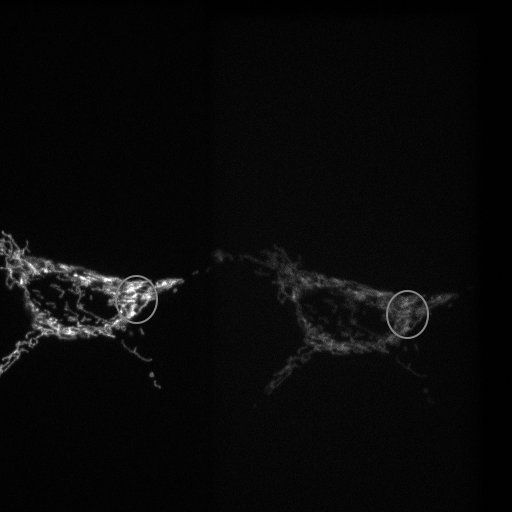
\includegraphics[width=0.9\textwidth]{Images/Green_to_red/5.jpg}
        \caption{Before}
    \end{minipage}%
    \begin{minipage}[t]{0.5\linewidth}
        \centering
        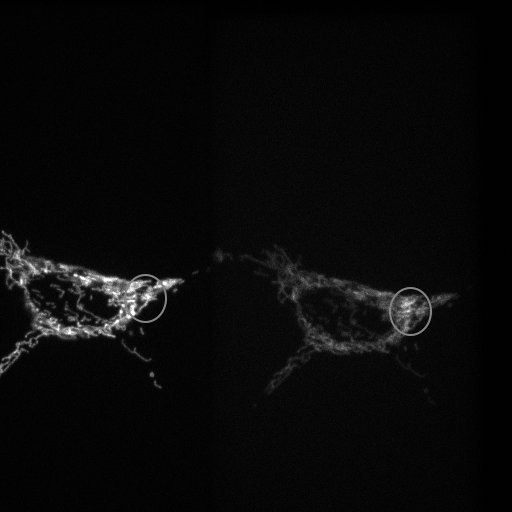
\includegraphics[width=0.9\textwidth]{Images/Green_to_red/20.jpg}
        \caption{After}
    \end{minipage}
    \caption{The cell images before and after applying the UV light(The white part is mitochondria, the circled part is the place UV light was applied)}
\end{figure}

The 5th frame(before applying UV) and the 20th frame(after applying UV) of the movie were shown in the Figure 4.3. In this figure, we could notice the intensity change of the mitochondrial fluorescence in the green(left) and red(right) channel. An obvious illumination increase at the circled point in the red channel. \\

By plotting the change of the mean intensity around the UV illuminated place by frames(Figure 4.4), we could spot that after the peak at around 10 frames, the green light has a slightly decrease, while the red light has a strong intensity increase, which means the photoconvertion from green to red happened in the mitochondria.


\begin{figure}[H]
    \centering
    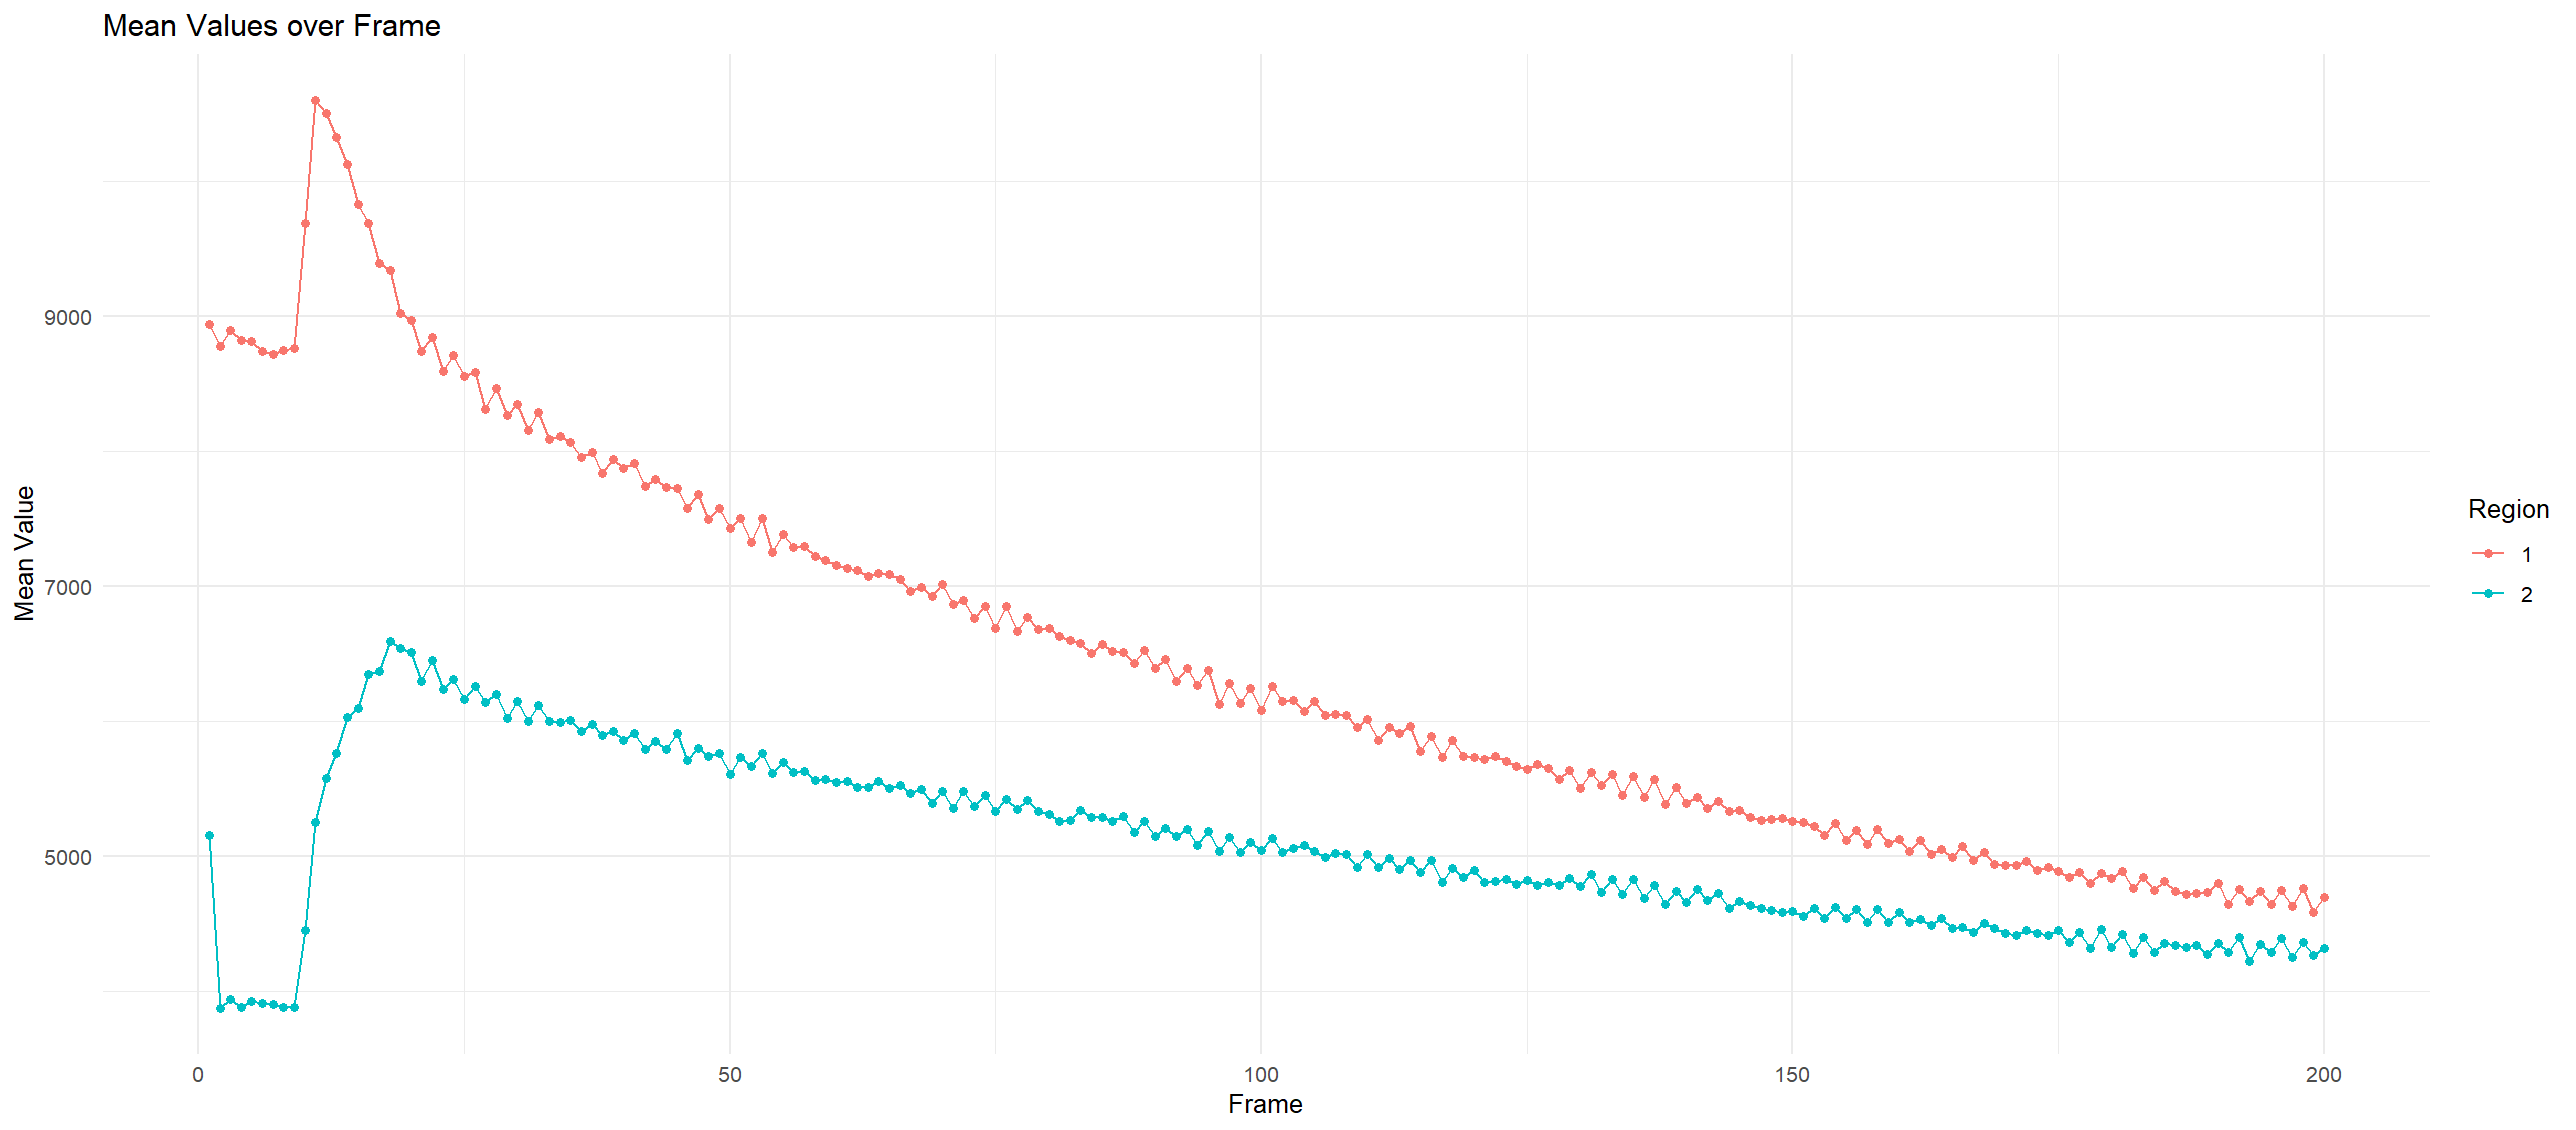
\includegraphics[width = 0.8\textwidth]{Images/Green_to_red/Intensity_Plot_DataEosFP-Mitochondria_dualCh_473nm+532nm.png}
    \caption{The mean intensity of the green light(up) and red light(down) by the frames(time)}
    \label{fig:enter-label}
\end{figure}


\section{Discussion}
% the mechanics how UV light makes the Photoconvert possible.
% the transmitted light into the red channels
In this experiment, we observed the green-to-red conversion of the EosFP in the mitochondria of live HeLa cells. The UV light could break the peptide backbone near the chromophore and an extension of the conjugated pi-electron system.\cite{EosFP} The UV exposure for such a localized and short time doesn't immediately lead to cell death \cite{UV_light}. With the help of this technique, we could observe the dynamic change of fluorophores in the living cell, in which ordinary fluorescence techniques would be impossible to record for the aforementioned time-resolution constraints.\\

After applying the green-yellow filter, we applied the green laser(532nm). Theoretically the red channel should not have any cell image at this moment. However, we could still observe a vague image of the mitochondria. That's because the filter could not filter out all the green lights. This will lead to an increase in the intensity of red light signal and a decrease in the intensity gap before and after the photoconversion. In this case, we can apply another filter before the red channel to filter the bleed-through light.

% figure 4.4 should show how 1 intensity gets lower while the other gets higher
Figure 4.4 shows how the relative intensity of region 1 displaying the emission in green has a rapid decrease after the UV conversion, and how region 2, displaying the red channel, has an inverse and proportional increase in intensity, highlighting the expected conversion and activity from the Eos Fluorescent Protein in the exposed region.
Figure 4.1 and 4.2 support this hypothesis as well.
%the graph that she showed us was normalized for intensity and it was much clearer, I remember it so I believe we should put it, since it´s the reason why we did this experiment...meaning tha even tough this graph doesn´t display it clearly it still holds true, and i believe she will ask why we didn´t note it in the discussion

%ah okay I put it in the experiment OTZ yeah but ithink it should be in the discussion. yeah okay
%it´s the experimental confirmation 
%so the conversion is green to red or yellow to red?
%green to red
%Yeah that's perfect, thank you!!! and next time if I write the discussion I will also put them main result in the discussion. That makes much sense
% I think we are done, Maybe I can print it out and sign?
% don´t worry we were far this afternoon and you couldn´t even discuss it with me 
% yeah, you wanna do my signature as well? Okay lol that's easier
%copy it from another report
% exactly
% Yeah!!!! LETSGOOOOO
\printbibliography
\end{document}